\subsection{Oversampling e Noise-Shaping}


\begin{frame}%[allowframebreaks]
  \frametitle{Oversampling e Noise-Shaping}
  Realizar uma sobre-amostragem (\textit{oversampling}) e, subsequente,
  uma filtragem passa-baixas discreta e uma decimação (\textit{down-sampling})
  permite uma redução no número de bits do quantizador, para uma mesma relação
  sinal-ruído-de-quantização (SQNR\footnote{Signal-to-Quantization-Noise Ratio}). 
  Mantendo número de bits do quantizador, é possível reduzir a SQNR.
\end{frame}

\begin{frame}[allowframebreaks]
  \frametitle{Conversão A/D com sobre-amostragem e quantização direta}
  Considere o sinal de entrada $x_a(t)$:
  \begin{itemize}
  \item média nula
  \item estacionário no sentido amplo 
  \item processo estocástico com densidade espectral de potência $\Phi_{x_a x_a}(j\Omega)$
  \item função de auto-correlação $\phi_{x_a x_a}(\tau)$
  \item limitado em frequência em $\Omega_N$: $\Phi_{x_a x_a}(j\Omega) = 0$, $\Omega \ge \Omega_N$
  \end{itemize}
  Vamos assumir que $2\pi / T = 2 M \Omega_N$. A constante inteira $M$ é o fator de sobre-amostragem.

  \framebreak 

  \begin{figure}[h!]
  \centering
  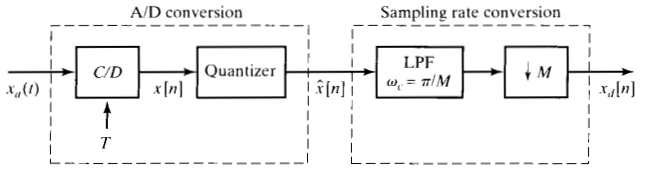
\includegraphics[width=0.8\textwidth]{images/oppenheim_fig456.png}
  \caption{Conversão A/D com sobre-amostragem \citep{oppenheim2009}.}
  \label{fig:oppenheim_fig456}
  \end{figure}

  \framebreak

  Utilizando o modelo do ruído aditivo.
  \begin{figure}[h!]
  \centering
  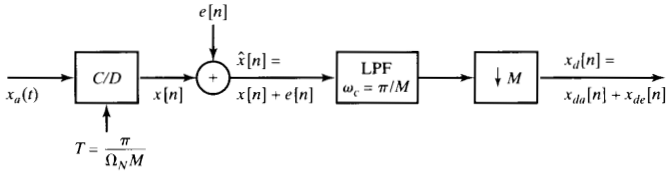
\includegraphics[width=\textwidth]{images/oppenheim_fig457.png}
  \caption{Modelo do ruído aditivo na conversão A/D com sobre-amostragem \citep{oppenheim2009}.}
  \label{fig:oppenheim_fig457}
  \end{figure}
  A saída $x_d[n]$ possui duas componentes: $x_{da}[n]$ (devido ao sinal $x_a(t)$) e $x_{de}[n]$ (devido ao ruído $e[n]$).

  Vamos analisar o efeito de cada componente na saída.

  \framebreak 

  Primeiramente vamos considerar o efeito da componente sinal.

  $\phi_{xx}[m]$ e $\Phi(e^{j\omega})$ são autocorrelação e densidade espectral de potência de $x[n]$, respectivamente.
  Por definição
  \begin{equation}
  \phi_{xx}[m] = \varepsilon\{x[n+m] x[n]\} .
  \end{equation}
  Como $x[n]=x_a(nT)$ e $x[n+m]=x_a(nT+mT)$
  \begin{equation}
  \label{eq-exp-xx}
  \varepsilon\{x[n+m] x[n]\} = \varepsilon\{x_a((n+m)T) x_a(nT)\} .
  \end{equation}
  Assim
  \begin{equation}
  \label{eq-phixxm}
  \phi_{xx}[m] = \phi_{x_a x_a} (mT)
  \end{equation}
  i.e., a função de autocorrelação da sequência de amostras é a versão amostrada da
  função de autocorrelação do sinal contínuo correspondente.

  \framebreak

  \Cref{eq-exp-xx,eq-phixxm}, juntamente com a suposição de estacionariedade no sentido amplo, levam a 
  \begin{equation}
  \varepsilon\{x^2[n]\} = \varepsilon\{x_a^2(nT)\} = \varepsilon\{x_a^2(t)\} \quad \textmd{ for all } n \textmd{ or } t.
  \end{equation}
  Como as densidades espectrais de potência são transformadas de Fourier das funções de autocorrelação,
  como consequência da \Cref{eq-phixxm} teremos
  \begin{equation}
  \label{eq-Phixx}
  \Phi_{xx}(e^{j\Omega T}) = \frac{1}{T} \sum_{k=-\infty}^{\infty} \Phi_{x_a x_a} \left( j \left( \Omega - \frac{2\pi k}{T} \right) \right) .
  \end{equation}

  \framebreak

  Assumindo um fator de sobre-amostragem $M$, tal que $2\pi/T = 2M\Omega_N$, substituindo $\Omega = \omega/T$ na \Cref{eq-Phixx}
  \begin{equation}
  \label{eq-Phixxiw}
  \Phi_{xx} (e^{j\omega}) = \begin{cases} \frac{1}{T} \Phi_{x_a x_a} \left( j \frac{\omega}{T} \right)   \quad & , |\omega| < \pi/M,  \\ 
  0 & , \pi/M < \omega \le \pi .\end{cases}
  \end{equation}
  
  \begin{figure}[h!]
  \centering
  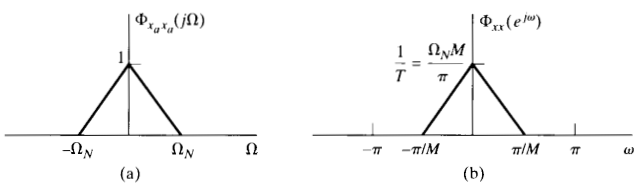
\includegraphics[width=0.7\textwidth]{images/oppenheim_fig458.png}
  \caption{Densidade espectral de potência \citep{oppenheim2009}.}
  \label{fig:oppenheim_fig458}
  \end{figure}

  \framebreak

  A potência total do sinal analógico é dada por
  \begin{equation}
  \varepsilon\{x_a^2(t)\} = \frac{2}{2\pi} \int_{-\Omega_N}^{\Omega_N} \Phi_{x_a x_a} (j \Omega) d\Omega .
  \end{equation}
  Pela \Cref{eq-Phixxiw}, a potência total do sinal amostrado é
  \begin{eqnarray}
  \varepsilon\{x^2[n]\} &=& \frac{1}{2\pi} \int_{-\pi}^{\pi} \Phi_{xx}(e^{j\omega}) d\omega \nonumber \\
                        &=& \frac{1}{2\pi} \int_{-\pi/M}^{\pi/M} \frac{1}{T} \Phi_{x_a x_a} \left( j \frac{\omega}{T} \right) d\omega \nonumber \\
                        &=& \frac{1}{2\pi} \int_{-\Omega_N}^{\Omega_N} \Phi_{x_a x_a} (j\Omega) d\Omega = \varepsilon\{x_a^2(t)\} ,
  \end{eqnarray}
  onde utilizamos $\Omega_N T = \pi/M$ e $\Omega = \omega/T$.
  Assim, a potência total do sinal amostrado é igual à potência total do sinal analógico.

  \framebreak
 
  Como $\Phi_{xx}(e^{j\omega})$ é limitado em frequência a $|\omega| < \pi/M$,
  \begin{eqnarray}
  \Phi_{x_{da} x_{da}} (e^{j\omega}) &=& \frac{1}{M} \sum_{k=0}^{M-1} \Phi_{xx} (e^{j(\omega - 2\pi k)/M}) \nonumber \\
                                     &=& \frac{1}{M} \Phi_{xx} (e^{j\omega /M})
  \end{eqnarray}
  A potência total da saída $x_{da}[n]$ é 
  \begin{eqnarray}
  \varepsilon\{x^2_{da}[n]\} &=& \frac{1}{2\pi} \int_{-\pi}^{\pi} \Phi_{x_{da} x_{da}} (e^{j \omega}) d\omega \nonumber = \frac{1}{2\pi} \int_{-\pi}^{\pi} \frac{1}{M} \Phi_{xx} (e^{j\omega/M}) d\omega \nonumber \\
                             &=& \frac{1}{2\pi} \int_{-\pi/M}^{\pi/M} \Phi_{xx} (e^{j\omega}) d\omega = \varepsilon\{x^2 [n]\} .
  \end{eqnarray}
  A potência total da componente de sinal permanece a mesma enquanto atravessa todo o sistema.

  \framebreak

  Considere agora a componente de ruído gerada pela quantização.
  Vamos assumir que $e[n]$ é ruído branco, estacionário no sentido amplo, e
  com variância 
  \begin{equation}
  \label{eq-variance-noise}
  \sigma_e^2 = \frac{\Delta^2}{12} .
  \end{equation}
  Consequentemente, a função de autocorrelação e densidade espectral de potência de $e[n]$
  são dadas, respectivamente, por
  \begin{equation}
  \label{eq-autocorr-noise}
  \phi_{ee} [m] = \sigma_e^2 \delta[m]
  \end{equation}
  e
  \begin{equation}
  \label{eq-power-density-noise}
  \Phi_{ee}(e^{j\omega}) = \sigma_e^2 \quad |\omega| < \pi .
  \end{equation}

  \framebreak

  \begin{figure}[h!]
  \centering
  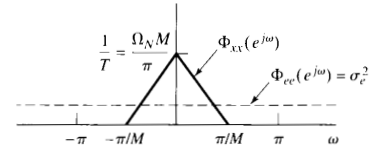
\includegraphics[width=0.7\textwidth]{images/oppenheim_fig459.png}
  \caption{Densidade espectral de potência do sinal e do ruído \citep{oppenheim2009}.}
  \label{fig:oppenheim_fig459}
  \end{figure}
  À medida que a taxa de sobre amostragem $M$ aumenta, menor será a parte do espectro do ruído
  de quantização que se sobreporá ao espectro do sinal.

  \framebreak

  O filtro passa-baixas ideal remove o ruído de quantização na banda  $\pi/M < |\omega| \le \pi$,
  enquanto deixa a componente de sinal inalterada.
  A potência do ruído na saída do filtro será
  \begin{equation}
  \varepsilon\{ e^2[n] \} = \frac{1}{2\pi} \int_{-\pi/M}^{\pi/M} \sigma_e^2 d\omega = \frac{\sigma_e^2}{M} .
  \end{equation}

  \framebreak

  \begin{figure}[h!]
  \centering
  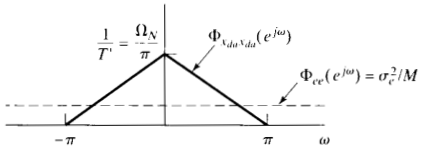
\includegraphics[width=0.75\textwidth]{images/oppenheim_fig460.png}
  \caption{Densidades espectrais de potência do sinal e ruído, após a decimação \citep{oppenheim2009}.}
  \label{fig:oppenheim_fig460}
  \end{figure}

  \begin{equation}
  \label{eq-qn-power-xde}
  \varepsilon\{ x^2_{de} \} = \frac{1}{2\pi} \int_{-\pi}^{\pi} \frac{\sigma_e^2}{M} d\omega = \frac{\sigma_e^2}{M} = \frac{\Delta^2}{12 M} .
  \end{equation}

  A potência do ruído de quantização $\varepsilon\{ x^2_{de} [n]\}$ reduziu por um fator $M$
  através do filtro e decimação, enquanto a potência do sinal permaneceu inalterada.

  \framebreak

  Utilizando \Cref{eq-qn-power-xde,eq-Xm-B} ($\Delta = X_m/2^B$),
  para uma dada potência de ruído de quantização, existe claramente uma relação
  de compromisso entre o fator de sobre-amostragem $M$ e o passo de quantização $\Delta$.
  \begin{equation}
  \label{eq-pne-MB}
  \varepsilon\{ x^2_{de} [n]\} = \frac{1}{12M} \left( \frac{X_m}{2^B} \right)^2 .
  \end{equation}
  Fixando o quantizador, a potência do ruído pode ser diminuída aumentando o fator de sobre-amostragem $M$.

  \framebreak

  Pela \Cref{eq-pne-MB}, fixando a potência do ruído de quantização $P_{de} = \varepsilon \{ x^2_{de} [n]\}$,
  \begin{equation}
  B = - \frac{1}{2} \log_2 M - \frac{1}{2} \log_2 12 - \frac{1}{2} \log_2 P_{de} + \log_2 X_m .
  \end{equation}
  Para cada vez que dobrarmos o fator de sobre-amostragem $M$, precisaremos de $1/2$ bit a menos
  para obter a mesma relação sinal-ruído-de-quantização 
  (para $M=4$ podemos utilizar um bit a menos e obter a mesma acurácia na representação do sinal).
\end{frame}

\begin{frame}[allowframebreaks]
  \frametitle{Conversão A/D com \textit{Noise Shaping}}
   a
\end{frame}

%\begin{frame}%[allowframebreaks]
%  \frametitle{}
%\end{frame}

%\begin{frame}%[allowframebreaks]
%  \frametitle{}
%\end{frame}

%\begin{frame}%[allowframebreaks]
%  \frametitle{}
%\end{frame}

%\begin{frame}%[allowframebreaks]
%  \frametitle{}
%\end{frame}

%\begin{frame}%[allowframebreaks]
%  \frametitle{}
%\end{frame}

%\begin{frame}%[allowframebreaks]
%  \frametitle{}
%\end{frame}


